\chapter{Semi Automatic Annotation} \label{chapter:semi_automatic}

\begin{figure}[!tbp]
	\centering
    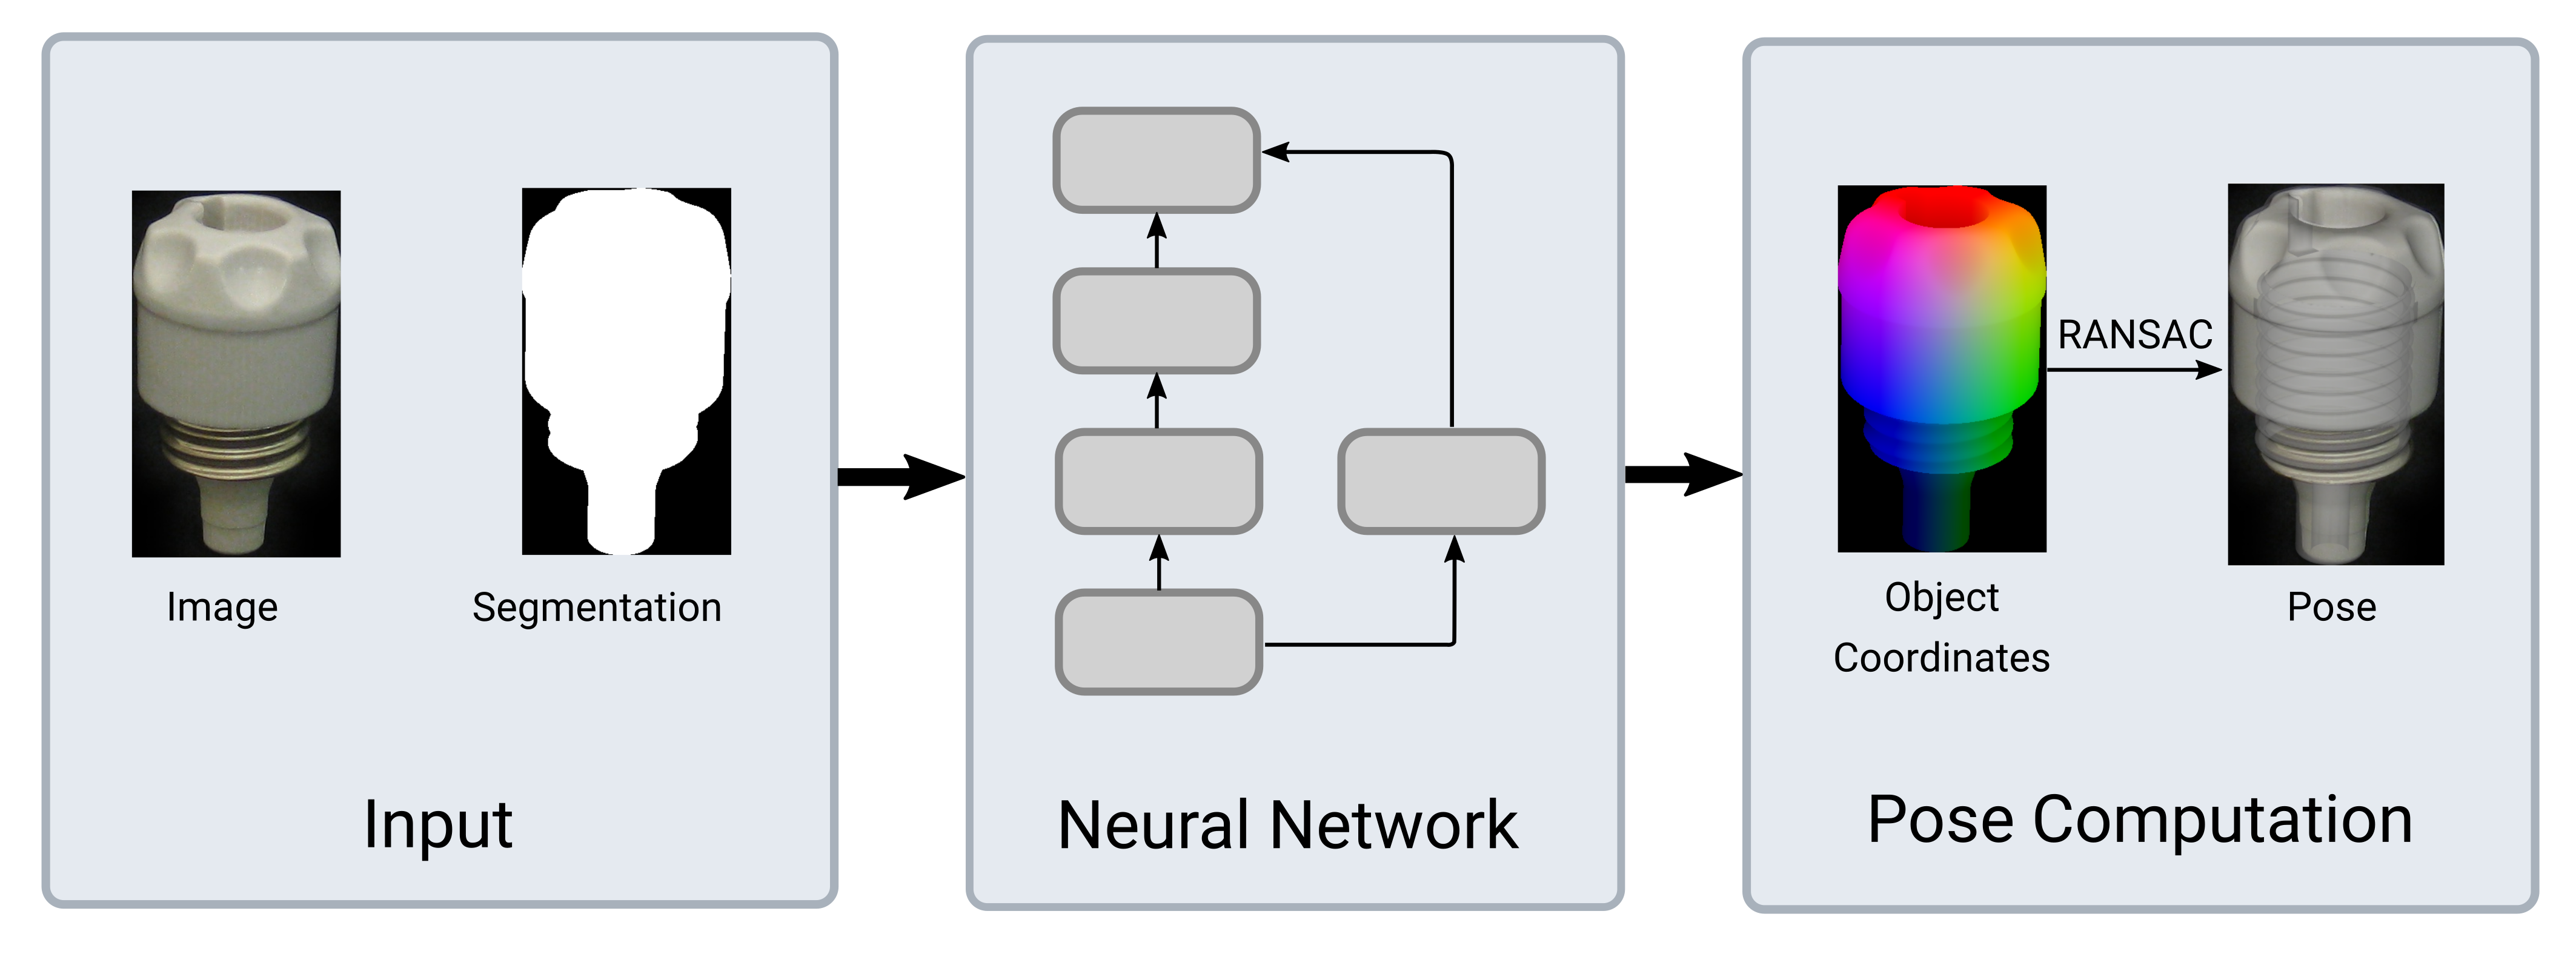
\includegraphics[width=\linewidth]{network_pipeline}
    \caption{The schematic pipeline of the neural network. The input to the network are the image and the corresponding segmentation image. The neural network then uses the segmentation to retrieve the pixels to predict object coordinates for. In the final pose computation stage the object coordinates and their 2D locations are used to retrieve the best pose using RANSAC. The object's transparency has been decreased to render the final pose. Own image.}
    	\label{fig:network_pipeline}
\end{figure} 

To assist in the process of manual image annotation presented in chapter \ref{chapter:manual_annotation}, we developed a neural network tailored to the task of 6D pose estimation with the medical images in mind. This chapter describes the network architecture and its variations, as well as different approaches to train the network and the modified annotation process resulting from the usage of the network.

\section{Terminology}

\noindent\textbf{Residual Connection.} A \textit{residual connection} (or skip connection) is a part of a neural network that skips some layers of the network and adds the input of a layer to the output of a layer that is situated deeper in the network. They can prevent the problem of the increasing training error in deeper networks. Fig. \ref{fig:residual_connection} visualizes such a connection. \\

\noindent\textbf{Depth Image.} A \textit{depth image} is an image $D$ that contains the distance $d$ of the camera to the surface for each pixel $u$ in an image $I$. Depth images can be created using special cameras or from stereo images and are often used in pose estimation and other computer vision tasks. A depth image can also be denoted by "RGB-D". \\

\noindent\textbf{Training Set.} A \textit{training set} is a subset of the dataset intended to train a neural network with. The training set is the set that the network actually uses to adjust its weights as opposed to the validation set. \\

\noindent\textbf{Training Example.} A \textit{training example} is an element from the training set fed to the neural network during training. \\

\noindent\textbf{Validation Set.} A \textit{validation set} is a subset of the dataset intended to train a neural network with. The validation set's purpose is to validate (thus the name) the networks new configuration which emerged from a run within the training. \\

\noindent\textbf{L1 Loss.} The \textit{L1 loss} is a loss function that sums up the absolute differences of the single elements, i.e. $L1(x, y) = \sum\limits_i |x_i - y_i|$. \\

\noindent\textbf{L2 Loss.} The \textit{L2 loss} is a loss function that sums up the squared differences of the single elements, i.e. $L2(x, y) = \sum\limits_i (x_i - y_i)^2$. \\

\noindent\textbf{L2 Regularization.} \textit{L2 regularization} penalizes the weights by a factor $\lambda$ in the following way: $\lambda \sum\limits_i w_i^2$. The regularization term is added to the weight update to keep the network from overfitting. \\

\noindent\textbf{Dropout Percentage.} \textit{Dropout percentage} is the percentage of neurons to deactivate of a layer. \\

\noindent\textbf{Receptive Field-Size.} The \textit{receptive field-size} of a network denotes how many input pixels an output value of the network has taken into account. This factor is determined by the number of operations in the network and their parameters. A convolution operation can skip pixels for example and the size of the layer's kernel can be adjusted, as well. A larger kernel results in more pixels used to compute one output value. Similarly, skipping pixels while the kernels still overlap, or at least no pixels are completely omitted in between, means that the receptive field size grows. The field size has to be adjusted to the problem.

\section{Network Architecture}

\begin{figure}[!tbp]
	\centering
	\begin{subfigure}[t]{0.47\textwidth}
		\centering
    	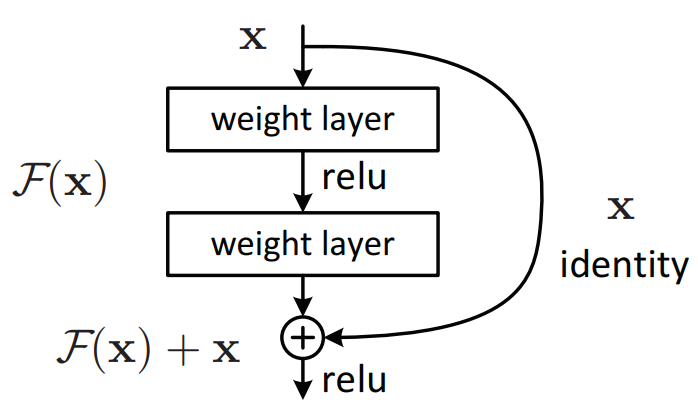
\includegraphics[width=\linewidth]{residual_connection}
    	\caption{A detailed view on a residual connection. The residual connections add the input of earlier layers of the network to deeper ones.}
    	\label{fig:residual_connection}
	\end{subfigure}
	\hfill
	\begin{subfigure}[t]{0.47\textwidth}
		\centering
    	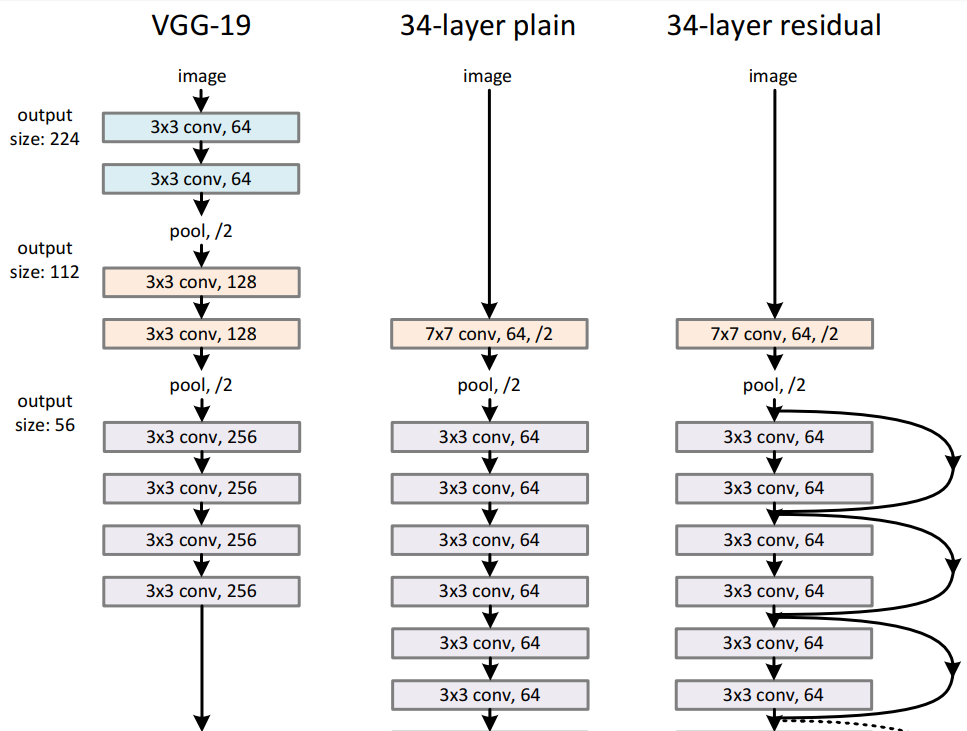
\includegraphics[width=\linewidth]{resnet_comparison}
    	\caption{Excerpt of a comparison between the ResNet architecture and VGG. The ResNet allows the creation of deeper network as the problem of vanishing gradients, i.e. very small gradients at deeper layers, can be targeted this way. The image has been cropped.}
    	\label{fig:resnet_comparison}
	\end{subfigure}
	\caption{A key component of ResNet: the residual connection. Left shows the connection in detail and right shows a comparison with the VGG architecture. Images from \cite{resnet}.}
	\label{fig:resnet_details}
\end{figure} 

The architecture of the network is adapted to the problem specific to the medical images. This means that the network expects segmentation masks as input together with the actual images. There is no mechanism of inferring the masks. This significantly reduces the complexity of predicting the position of the object, although object coordinates implying different poses can still lead to significant errors. This precondition yielded to the pipeline visible in fig \ref{fig:network_pipeline} which takes the actual image and the segmentation image as input. The images shown are already cropped to the segmentation mask but in later applications the image size and proportion of pixels belonging to the object can be arbitrary. It is important to note that the network does not take depth images as input opposed to many other pose estimation approaches. This is owed to the nature of the provided medical images which do not contain depth information. The network then processes each pixel which is part of the object according to the segmentation image and outputs the 3D coordinates. As explained in chapter \ref{chapter:background} we then compute the optimal pose using RANSAC and the 2D-3D correspondences.

The basic architecture that we chose for the network is called ResNet. ResNet was first presented in \cite{resnet} and enabled researchers to create deeper networks than before. Two major problems arise with very deep neural networks. The vanishing gradients problem, which occurs in deeper networks, means that gradients gradually become 0 in later layers. This can problem be targeted with batch normalization. The second problem of an increasing training error the deeper the network becomes can be solved using ResNet (or flavors of it). Adding layers to a network to increase expressivity does not directly lead to a higher accuracy. Even stacking identity layers, i.e. layers that learn the mathmatical identity function $f(x) = x$, ontop of the network increases the training error. This phenomenom can be partly compensated with residual connections \cite{resnet}. An example of a residual connection can be seen in fig. \ref{fig:residual_connection}. Fig. \ref{fig:resnet_comparison} shows a comparison of ResNet with the architecture \textit{VGG} \cite{vgg}. The residual connections are clearly visible as the arcs of the rightmost architecture. ResNet has proven to produce reliable and accurate results in many computer vision tasks.

The basic structure of the network can be seen in fig. \ref{fig:network_architecture}. The recurring blocks are the building blocks of the network and consist of three convolutions on the long path (the left part of the block) and depending of the type of block, i.e. convolution or identity block, the right path directly adds the identity to the output or performs another convolution before the addition. The number of operations on both paths is higher than the number of convolutions only because activations and batchnormalization are added, as well.

\subsection{Loss \& Optimizer}

Since the network outputs the 3D coordinates for each pixel in the input image the straight-forward approach is to penalize the differences with respect to the ground-truth coordinates. The loss function sums up the absolute differences of the individual XYZ components of the predicted object coordinate and the ground-truth, but only at the relevant positions according to the segmentation mask. This is the L1 loss. The reason why we chose the L1 loss over the L2 loss is that the L2 loss penalizes outliers more but outliers potentially get eliminated in the \gls{ransac} algorithm during pose computation. We used L2 regularization for the weights. Due to its performance (see chapter \ref{chapter:experiments}), we selected Adam as the optimizer for all networks.

\subsection{Variations} \label{section:network_variations}

\begin{figure}[!tbp]
	\centering
    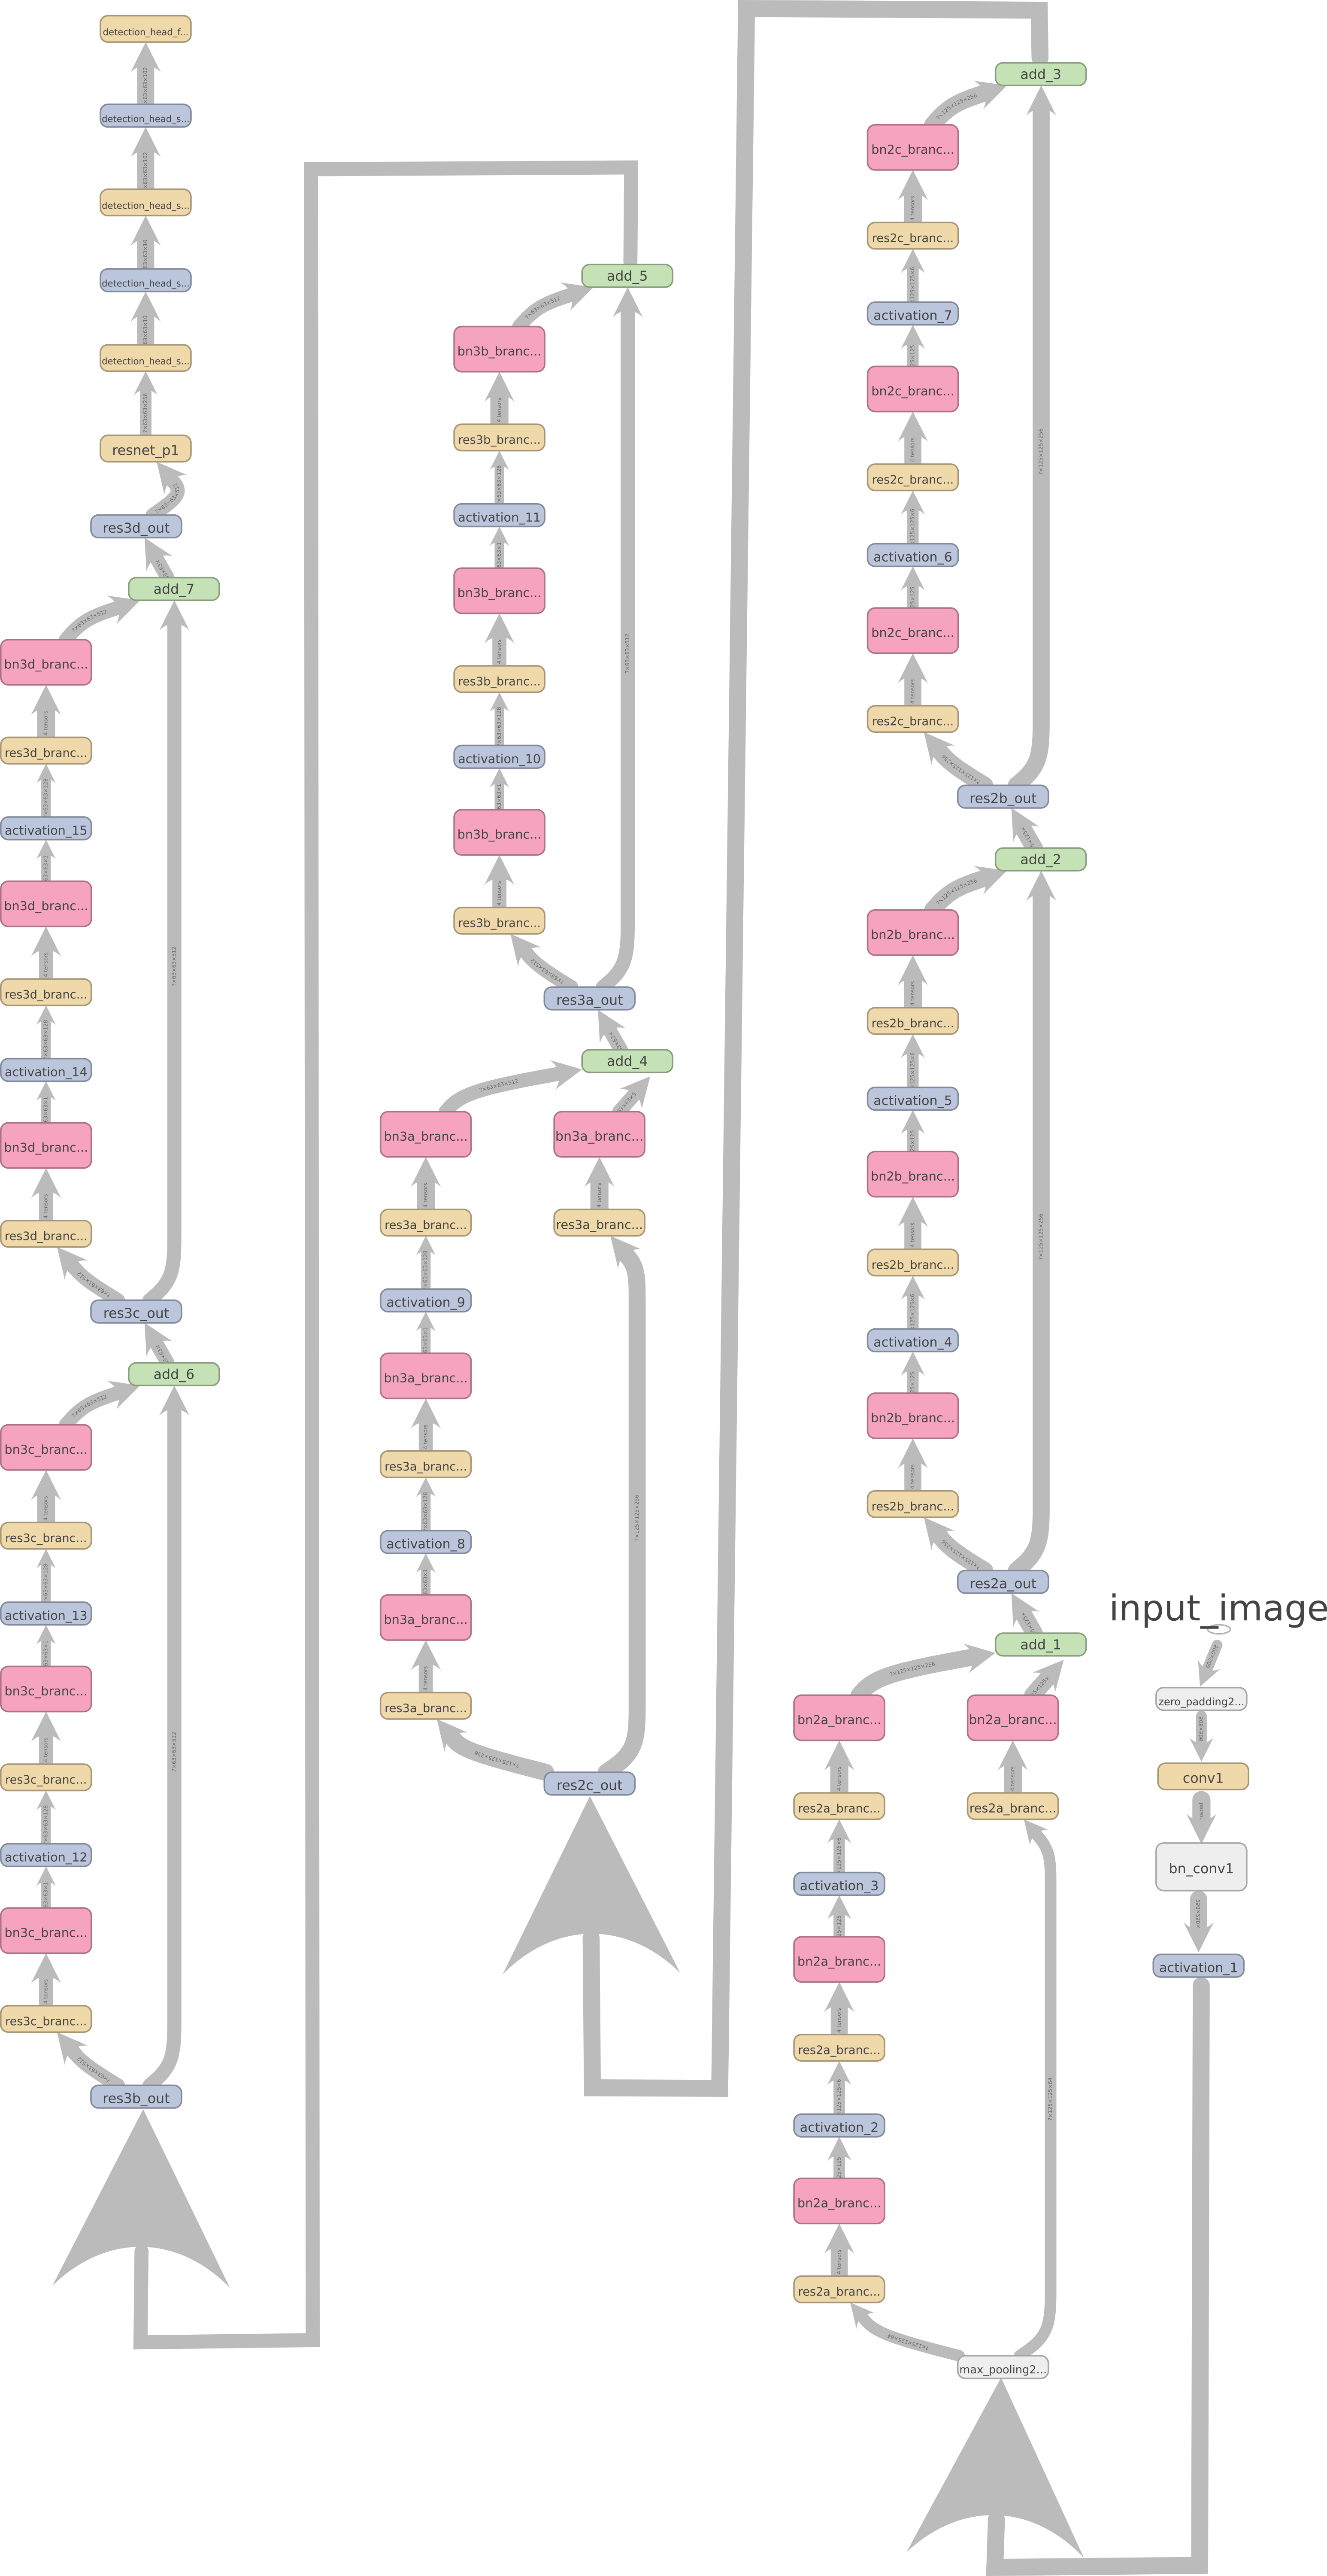
\includegraphics[width=0.75\linewidth]{network_architecture}
    \caption{An overview of the shallower architecture used in the project. The visualization was created using \textit{Tensorboard} but modified to fit one page. The large arrows have no meaning and are only there to emphasize where the network continues. Own image.}
    	\label{fig:network_architecture}
\end{figure}

To find the optimal network structure a total of 6 network architectures were created and later compared in chapter \ref{chapter:experiments}. The first design of the network consisted of 23 convolutional layers with a receptive field-size of 99. A characteristic of the medical images is that the tools have writings on them which is often not or only partly visible. This is the reason why we reduced the field-size to keep the network from detecting poses based and the letters. Due to the complications described in section \ref{section:6dpat_difficulties} annotating the medical images was not possible and we were thus not able to fully prove our statement. The second architecture added more layers to a total of 35, while decreasing the receptive field-size to 67. The third architecture kept the number of layers of the first but reduced the field-size to 51. We also created three deeper networks of 50 layers, of which two omit bachtnormalization and use dropout instead, both with a receptive field-size of 59. The difference between the two is the number of dropout-layers and the dropout percentage. The third still employs batchnormalization, again with a receptive field-size of 59.

\section{Implementation}

The neural network and all of its utility functionality is implemented in Python using Tensorflow \cite{tensorflow} and Keras \cite{keras}. Tensorflow is a deep-learning framework that uses C++ do perform the actual calculations. It provides many different layers, as well as tools to modify images, automatic differentiation of the loss function and a lot of other functionality. Keras is a framework that makes using Tensorflow easier by providing even higher-level access and allows to create neural network in a few lines of code. Because most operations of a neural network written in Tensorflow and Keras are performed using C++ code and because computation can be transferred to the GPU at nearly no extra effort, such a network is considerably faster than an implementation in Python might imply.

\section{Modes of Operation} \label{section:modes_of_operation}

The goal of the neural network is to make the annotation process presented in chapter \ref{chapter:manual_annotation} faster and more efficient. To achieve this we strove for a symbiosis between the annotation tool and the neural network. The new workflow is visualized in fig. \ref{fig:semi_automatic_workflow}. In addition to manually annotate images, a user can use the annotated images to train the neural network. After training the neural network, the user can run the network on new images to predict poses and correct them with the aid of the annotation tool. The improved pose predictions can serve as input to further train the network. There are two main strategies of training a neural network that we will consider here. Those two are training from scratch and an incremental training approach.

\begin{figure}[!tbp]
	\centering
    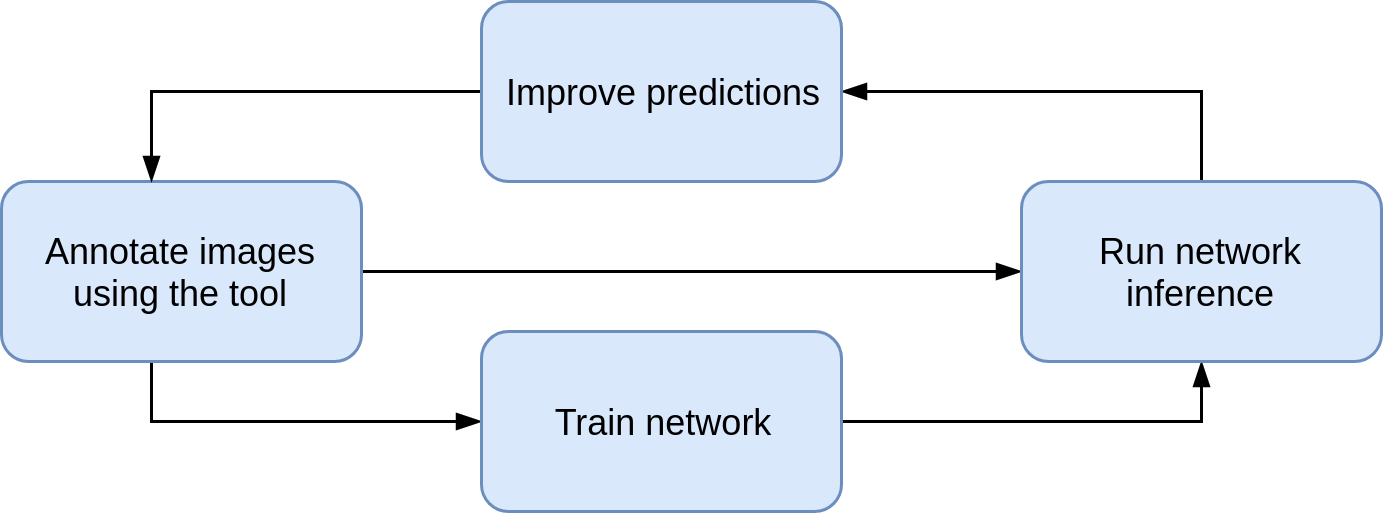
\includegraphics[width=0.75\linewidth]{semi_automatic_workflow}
    \caption{The new workflow of the annotation procedure including the neural network. First, the user has to annotate enough images from the dataset to be able to train the network. After successfully training the network it can be used to predict poses on a subset of the dataset. The user can then improve the poses and return to annotating more images or run the network inference on more images. Own image.}
    	\label{fig:semi_automatic_workflow}
\end{figure}

\noindent\textbf{Training from Scratch.} \textit{Training from scratch} describes the method of training the network with all images (usually divided into training and validation set) and initializing  the weights of the network to 0 or randomly. This procedure requires a lot of time as all images of the already annotated ones have to be processed. It also requires many training examples but can on the other hand work with uninitialized weights.

\noindent\textbf{Incremental Training.} \textit{Incremental training} can be performed when the user has already annotated some images and trained the network to some extend. After more images have been annotated the network is trained again. But instead of training from scratch, the pre-trained weights are used as the initial weights and the network is fed examples from the freshly annotated images. This process is usually finishes faster, as the network gets to see fewer training examples but requires that the user trained the weights of the network already to some extend.

\noindent\textbf{Inference.}  After training the network using one of the two training strategies, it can be used to predict poses on unseen images. To amortize the time needed to load the weights of the network it is best to run inference for many images and not only one. The network inference can be directly called from the annotation tool that we presented in chapter \ref{chapter:manual_annotation}.